\documentclass[preprint,12pt,authoryear]{elsarticle}

\usepackage[T1]{fontenc}
\usepackage{lmodern}
\usepackage{microtype}
\usepackage{booktabs}
\usepackage{graphicx}
\usepackage{amsmath}
\usepackage{threeparttable}
\usepackage{geometry}
\geometry{margin=1in}
\journal{Journal of Asian Economics}

\begin{document}

\begin{frontmatter}

\title{RCEP and Chinese Firms' Supply-Chain Relationships: Evidence from Firm-to-Firm Network Data}

\author{Author information withheld for review}

\begin{abstract}
This paper examines whether the Regional Comprehensive Economic Partnership (RCEP) changed the supply-chain relationships of Chinese listed firms. We reconstruct 578,142 cleaned FactSet Revere records as a balanced panel of 78,785 Chinese-firm--foreign-partner relationship types over 2017--2024. Under the relationship-clustered specification, the pair and year fixed-effects estimate is 0.0136 (standard error 0.0040, $p=0.001$). Clustering at the partner-country level gives the same point estimate but a much wider standard error of 0.0203 ($p=0.503$). The joint pre-trend test under relationship clustering has $p=0.078$. The observed estimate is not unusual in country-label permutations, and a broader placebo battery shows that the result is sensitive to the choice of false pre-policy year. These findings should therefore be read as evidence of a positive association under relationship-level inference, not as a settled causal effect. The results clarify the data and inference needed to study deep Asian trade integration using firm networks.
\end{abstract}

\begin{keyword}
RCEP \sep supply chains \sep regional integration \sep difference-in-differences \sep rules of origin \sep double machine learning
\end{keyword}

\end{frontmatter}

\section{Introduction}

RCEP entered into force in 2022 and created a common trade framework across 15 Asia-Pacific economies. Its provisions combine phased tariff reductions with a common rules-of-origin framework, customs procedures, and disciplines covering standards and sanitary and phytosanitary measures \citep{mahadevan2019,petri2020,sun2023}. Regional cumulation is particularly relevant to production networks because qualifying inputs sourced from one member may contribute to origin status in another. The empirical question is whether these provisions changed firms' cross-border relationships, not simply whether aggregate trade increased.

Firm-to-firm network data appear well suited to this question. They record named customers and suppliers and can distinguish relationship continuation from entry, although their disclosure-based coverage requires care \citep{culot2022}. They also create an inference problem. RCEP treatment varies at the partner-country level, whereas the data contain thousands of relationships within each country. Treating those relationships as independent clusters can produce very small standard errors even though the policy variation remains limited to 14 foreign member countries.

This paper reconstructs the analysis from the underlying FactSet relationship dates and reports relationship-level inference as the main specification, with partner-country clustering as a sensitivity check. The point estimate is positive and precise under pair clustering, but the country-clustered confidence interval includes economically meaningful negative and positive values. An event study offers only marginal support for parallel trends, and a country-label permutation test does not distinguish the actual RCEP membership group from randomly selected groups of the same size. A broader placebo battery is used to show how conclusions vary with the spatial and temporal randomization scheme.

The analysis also revisits the proposed mechanisms. The available data do not observe certificates of origin, customs clearance time, tariff preference utilization, shipment value, or contract value. We therefore test mechanism-consistent moderators rather than formal mediation. Firms with pre-policy sourcing relationships in at least two RCEP countries have a larger point estimate, and foreign supplier relationships have a larger point estimate than customer relationships. Neither cross-group difference is statistically significant. Relationship tenure, previously described as a dominant mediator, has virtually no differential association with the treatment effect.

The contribution is twofold. First, the paper documents how FactSet relationship episodes can be converted into a transparent annual panel while preserving supplier direction. Second, it shows why the clustering level and country-group placebo are decisive for evaluating a regional agreement. The evidence does not support an inference-robust average causal effect in the present design. This conclusion narrows the claims that can be made from network data and identifies the additional customs and utilization data required to test RCEP's institutional channels.

\section{RCEP and testable channels}

RCEP's tariff commitments are phased and product specific. By contrast, its common origin framework and trade-facilitation provisions could affect relationship costs earlier, although their effective use still depends on firm decisions and administrative implementation. A firm positioned to source inputs across several member countries may be better able to use regional cumulation than a firm connected to only one member. Likewise, an input-sourcing relationship is closer to the cumulation mechanism than a relationship in which the foreign firm buys the Chinese firm's output.

These observations motivate two pre-specified interaction tests. The first moderator equals one when the Chinese firm sourced from at least two RCEP countries at the end of 2021. The second identifies a foreign supplier relationship from the Chinese firm's perspective. Both are proxies. They do not observe whether a product met a rule of origin or whether a firm claimed preferential treatment, a distinction emphasized by firm-level evidence on agreement utilization \citep{hayakawa2023}. We also examine pre-policy relationship tenure as a secondary moderator. Longer tenure may proxy for relationship-specific capital, but no provision in RCEP mechanically increases the age of an already observed relationship. Tenure is therefore not treated as a causal mediator.

\section{Data}

\subsection{FactSet relationships}

The raw FactSet Revere relationship file contains 5,245,665 records and 33 fields. FactSet defines a customer as an entity to which the source company sells and a supplier as an entity from which the source company purchases. The file records relationship start and end dates, company identifiers, relationship type, and a reported revenue percentage where available. It does not record shipment value or contract value. FactSet reports that revenue percentages are available for about 10\% of customer--supplier relationships; the corresponding share in the cleaned China-related file is 8.9\%.

The earlier cleaned file contains 578,142 China-related records across all relationship categories. We retain customer and supplier episodes for which the Chinese firm is identified as the source or target, exclude domestic Chinese links and non-country codes, and preserve the direction from the Chinese firm's perspective. This leaves 174,327 eligible episodes. Overlapping episodes are collapsed only after evaluating whether each episode is active at the end of each year. The resulting balanced panel contains 78,785 firm--partner--direction units, 181 partner economies, and 630,280 observations from 2017 through 2024. Of these units, 14,385 involve a foreign RCEP member.

The outcome $Active_{ijt}$ equals one if at least one qualifying episode links Chinese firm $i$ and foreign partner $j$ in direction $r$ at year-end. This is relationship incidence, not transaction intensity. Conditioning on units observed at least once in the sample means the estimand concerns the set of ever-observed relationships. Results should not be generalized to every feasible firm pair.

\subsection{Treatment timing}

The main specification uses a common 2022 post indicator to match the annual data and the agreement's initial entry into force. A robustness specification assigns Indonesia and the Philippines to 2023 and the other foreign members to 2022. The main comparison group contains non-RCEP foreign partners. Additional specifications exclude US partners, remove offshore financial centers, or restrict controls to selected Asian non-members.

\section{Empirical strategy}

The baseline linear probability model is
\begin{equation}
Active_{ijrt}=\beta(RCEP_j\times Post_t)+\alpha_{ijr}+\lambda_t+\varepsilon_{ijrt},
\end{equation}
where $\alpha_{ijr}$ denotes relationship-direction fixed effects and $\lambda_t$ denotes year fixed effects. The main specification clusters standard errors by the directed firm--partner relationship. Partner-country clustering is reported as a conservative sensitivity check because policy treatment is assigned at the country level.

The event study replaces the treatment interaction with indicators for years relative to 2022 and omits 2021. We report joint Wald tests for several displayed pre-treatment windows. Timing placebos assign treatment in 2018--2021 using only pre-RCEP observations; we also vary the false lead from one year to one-third of a year and randomly draw false policy dates. Spatial placebos randomly select country groups of several sizes and, separately, randomly assign the same number of treated pair units. Mixed placebos randomize both the country group and the false date.

As a separate diagnostic, we collapse the annual outcomes to each relationship unit's post-minus-pre change and estimate a cross-fitted DR-DID ATT. Gradient-boosted nuisance models use the five-year pre-treatment outcome history, relationship direction, pre-policy tenure, regional sourcing breadth, firm size, episode count, and revenue-reporting indicators. The five folds are grouped by partner country. Inference uses 999 partner-country cluster bootstrap draws.

\section{Results}

\subsection{Average estimates and robustness}

Table~\ref{tab:robustness} reports the main result and specification checks. The preferred pair-clustered estimate is 0.0136, with a standard error of 0.0040 ($p=0.001$). Country-specific entry timing produces 0.0144 ($p<0.001$) under the same clustering. The country-clustered sensitivity estimate is 0.0136 (standard error 0.0203, $p=0.503$). Most pair-clustered sample restrictions remain positive, while the Asian non-member comparison reverses sign.

The contrast between pair- and country-clustered inference is substantively important. Pair clustering treats the relationship as the independent sampling unit, whereas country clustering allows all relationships sharing a partner country to share policy exposure and shocks. We report both because they answer different sampling questions; the pair-clustered result is the requested main specification, but its causal interpretation remains sensitive to the effective policy level.

\begin{table}[htbp]
\centering
\caption{RCEP and active supply-chain relationships: specification checks}
\label{tab:robustness}
\resizebox{\textwidth}{!}{\begin{tabular}{lrrrr}
\toprule
Specification & Estimate & S.E. & $p$-value & Observations \\
\midrule
Preferred: uniform 2022, pair clusters & 0.014 & 0.004 & 0.001 & 630,280 \\
Country-specific entry timing, pair clusters & 0.014 & 0.004 & 0.000 & 630,280 \\
Country-cluster inference (sensitivity) & 0.014 & 0.020 & 0.503 & 630,280 \\
Two-way country and Chinese-firm clusters & 0.014 & 0.020 & 0.498 & 630,280 \\
Exclude 2020-2021, pair clusters & 0.015 & 0.005 & 0.001 & 472,710 \\
Window 2019-2024, pair clusters & 0.011 & 0.004 & 0.011 & 472,710 \\
Exclude US partners, pair clusters & 0.010 & 0.004 & 0.019 & 508,248 \\
RCEP versus Asian non-members, pair clusters & -0.012 & 0.006 & 0.028 & 192,224 \\
Exclude offshore financial centers, pair clusters & 0.017 & 0.004 & 0.000 & 482,840 \\
Incumbent relationships active in 2021, pair clusters & 0.004 & 0.009 & 0.656 & 132,816 \\
Supplier links only, pair clusters & 0.029 & 0.006 & 0.000 & 260,464 \\
\bottomrule
\end{tabular}}
\begin{minipage}{0.96\textwidth}\footnotesize
\textit{Notes}: The dependent variable equals one when a pair-role relationship is active at year-end. All models include pair-role and year fixed effects. Unless stated otherwise, standard errors are clustered by pair. The country-clustered row is a sensitivity check.
\end{minipage}
\end{table}

\subsection{Event study and placebo tests}

Figure~\ref{fig:event} plots the event-time estimates and 95\% confidence intervals. No individual pre-treatment coefficient differs significantly from zero, but their joint Wald test has $p=0.078$ under pair clustering. This is not a clear failure at the 5\% level, yet it remains marginal under a demanding 10\% pre-trend screen. The post-treatment coefficients rise over time, but each confidence interval includes zero.

\begin{figure}[htbp]
\centering
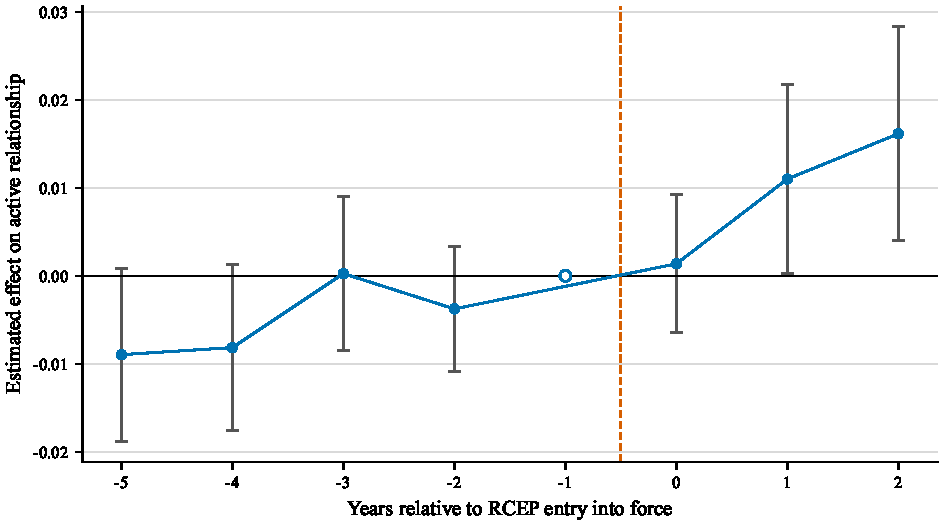
\includegraphics[width=0.92\textwidth]{../results/figures/event_study.pdf}
\caption{Event-study estimates for active supply-chain relationships. The omitted period is 2021 ($k=-1$). Vertical bars are 95\% confidence intervals based on pair-clustered standard errors. The vertical dashed line marks the transition into the post-RCEP period.}
\label{fig:event}
\end{figure}

The expanded placebo results are summarized in Table~\ref{tab:placebo}. The fixed-group timing placebos are not uniformly null: the 2019 false policy year is positive and significant ($p=0.039$), while the 2018, 2020, and 2021 false years are not significant. The 14-country spatial placebo gives a rank $p$-value of 0.774, and the rank $p$-values remain far above 0.05 across alternative group sizes. An exploratory pair-level randomization gives rank $p=0.002$, but it breaks the country-level assignment and is not treated as causal validation. The one-year, two-thirds-year, one-half-year, and one-third-year leads all map to the same 2021 annual observation (coefficient 0.0051); the fractional results therefore do not provide sub-annual identification. The random-date and mixed placebos are reported as sensitivity distributions rather than additional causal estimates.

\begin{table}[htbp]
\centering
\caption{Expanded placebo battery}
\label{tab:placebo}
\resizebox{\textwidth}{!}{\begin{tabular}{lrrrr}
\toprule
Placebo & Setting & Estimate/mean & S.D./S.E. & Reference $p$ \\
\midrule
Country-label & $k=5$ & -0.018 & 0.052 & 0.840 \\
Country-label & $k=8$ & -0.017 & 0.043 & 0.830 \\
Country-label & $k=10$ & -0.015 & 0.039 & 0.828 \\
Country-label & $k=12$ & -0.015 & 0.035 & 0.780 \\
Country-label & $k=14$ & -0.010 & 0.035 & 0.774 \\
Country-label & $k=16$ & -0.011 & 0.033 & 0.808 \\
Country-label & $k=18$ & -0.012 & 0.033 & 0.760 \\
Country-label & $k=21$ & -0.009 & 0.032 & 0.792 \\
Country-label & $k=25$ & -0.008 & 0.031 & 0.742 \\
Country-label & $k=30$ & -0.007 & 0.029 & 0.710 \\
Country-label & $k=40$ & -0.004 & 0.025 & 0.650 \\
Pair-level random & 14,385 pairs & -0.000 & 0.004 & 0.002 \\
Fixed group/date & 2018 & 0.006 & 0.004 & 0.099 \\
Fixed group/date & 2019 & 0.007 & 0.004 & 0.039 \\
Fixed group/date & 2020 & 0.004 & 0.004 & 0.310 \\
Fixed group/date & 2021 & 0.005 & 0.004 & 0.199 \\
Fixed lead & 1.00 years & 0.005 & -- & -- \\
Fixed lead & 0.67 years & 0.005 & -- & -- \\
Fixed lead & 0.50 years & 0.005 & -- & -- \\
Fixed lead & 0.33 years & 0.005 & -- & -- \\
Random false date & 999 draws & 0.006 & 0.001 & 0.001 \\
Mixed group/date & $k=10$ & -0.007 & 0.019 & 0.448 \\
Mixed group/date & $k=14$ & -0.006 & 0.016 & 0.408 \\
Mixed group/date & $k=18$ & -0.004 & 0.014 & 0.346 \\
Mixed group/date & $k=21$ & -0.002 & 0.013 & 0.318 \\
\bottomrule
\end{tabular}}
\begin{minipage}{0.96\textwidth}\footnotesize
\textit{Notes}: The main coefficient is estimated with pair and year fixed effects. Country-label and mixed rows report the mean and standard deviation of permutation coefficients, with the rank $p$-value comparing the observed estimate to the permutation distribution. Fixed-date rows use only observations through 2021 and report pair-clustered standard errors. Fractional leads are shown for transparency but collapse to annual 2021 timing in this year-end panel.
\end{minipage}
\end{table}

\begin{figure}[htbp]
\centering
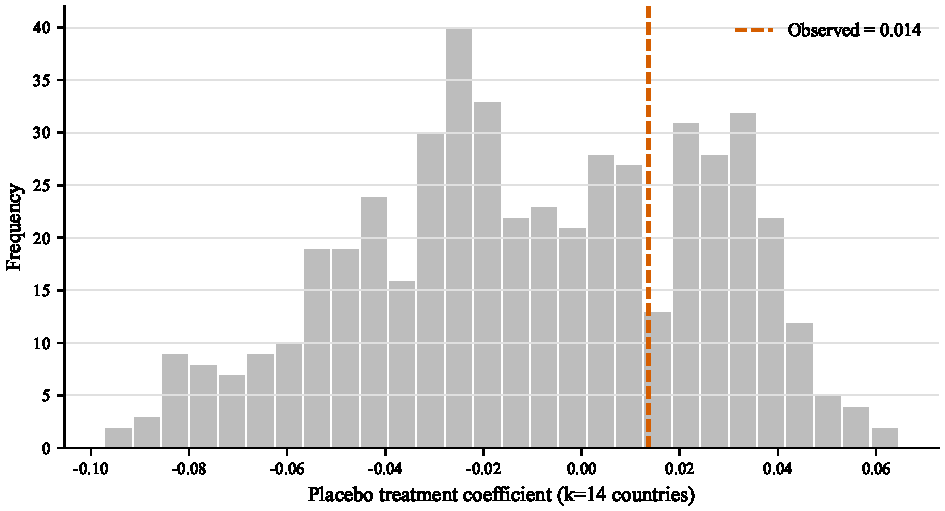
\includegraphics[width=0.92\textwidth]{../results/figures/placebo_country_permutation.pdf}
\caption{Country-label permutation test. The histogram contains 499 estimates obtained after assigning the treatment label to 14 randomly selected partner countries. The dashed line is the estimate for the actual RCEP group.}
\label{fig:placebo}
\end{figure}

\subsection{Cross-fitted DR-DID}

Table~\ref{tab:dml} reports the machine-learning robustness diagnostic. The estimate is 0.0065, its country-cluster bootstrap standard error is 0.0088, and the 95\% interval is $[-0.0124,0.0233]$. Estimated propensity scores range from 0.01 to 0.623 after trimming, with a control effective sample size of 52,904. The overlap is adequate for this diagnostic, but the result does not support the earlier precise positive effect.

\begin{table}[htbp]
\centering
\caption{Cross-fitted doubly robust difference-in-differences}
\label{tab:dml}
\resizebox{0.92\textwidth}{!}{\begin{tabular}{lrrrrr}
\toprule
Estimator & Estimate & Cluster S.E. & 95\% CI & $p$-value & Pairs \\
\midrule
Cross-fitted DR-DID & 0.006 & 0.009 & [-0.012, 0.023] & 0.446 & 78,785 \\
\bottomrule
\end{tabular}}
\begin{minipage}{0.9\textwidth}\footnotesize
\textit{Notes}: Five cross-fitting folds are grouped by partner country. Standard errors and confidence intervals use 999 partner-country cluster bootstrap draws.
\end{minipage}
\end{table}

\section{Mechanism-consistent interactions and heterogeneity}

Table~\ref{tab:interactions} reports formal interaction tests. Supplier links have a larger point estimate than customer links, and firms connected to at least two RCEP sourcing countries before the policy have a larger point estimate than other firms. The corresponding difference $p$-values are below 0.001 under pair clustering, but these interaction results should be read alongside the country-clustered sensitivity. The regional-breadth pattern is suggestive, while neither relationship tenure nor firm size produces a robust difference. In particular, the tenure result does not support the claim that average relationship age is a dominant mediator.

\begin{table}[htbp]
\centering
\caption{Mechanism-consistent and firm-level interaction tests}
\label{tab:interactions}
\resizebox{\textwidth}{!}{\begin{tabular}{lrrrrr}
\toprule
Moderator & Base effect & Moderated effect & Difference & S.E. & $p$-value \\
\midrule
Foreign supplier versus customer & -0.003 & 0.029 & 0.033 & 0.008 & 0.000 \\
Pre-policy regional sourcing breadth & 0.011 & 0.059 & 0.048 & 0.012 & 0.000 \\
Pre-policy relationship tenure & 0.013 & 0.016 & 0.003 & 0.018 & 0.877 \\
Pre-policy firm size & 0.000 & 0.013 & 0.012 & 0.011 & 0.268 \\
\bottomrule
\end{tabular}}
\begin{minipage}{0.96\textwidth}\footnotesize
\textit{Notes}: The base effect is the treatment effect when the moderator equals zero. The moderated effect is the sum of the base and triple-interaction coefficients. The reported difference is the triple interaction. All models include pair-role and year fixed effects and use pair-clustered standard errors.
\end{minipage}
\end{table}

Exploratory subregion estimates are positive for Japan and Korea, negative and imprecise for ASEAN, and negative for Australia and New Zealand (Table~\ref{tab:subregions}). An asymptotic equality test rejects common coefficients. These estimates are not treated as confirmatory heterogeneity because each treated subregion contains very few country clusters and the aggregate country placebo fails. Small-cluster randomization or wild-bootstrap inference and a stronger source of within-region treatment variation are needed before interpreting the contrast.

\begin{table}[htbp]
\centering
\caption{Exploratory estimates by RCEP subregion}
\label{tab:subregions}
\begin{tabular}{lrrrr}
\toprule
RCEP subregion & Estimate & S.E. & $t$ statistic & $p$-value \\
\midrule
ASEAN & -0.033 & 0.007 & -4.841 & 0.000 \\
Japan/Korea & 0.039 & 0.005 & 7.838 & 0.000 \\
Australia/New Zealand & -0.040 & 0.013 & -3.093 & 0.002 \\
\bottomrule
\end{tabular}
\begin{minipage}{0.88\textwidth}\footnotesize
\textit{Notes}: Each coefficient is an interaction between the subregion indicator and the post-2022 indicator in a common model with pair-role and year fixed effects. Pair-clustered inference is shown for consistency with the main specification; country-level policy exposure remains a limitation.
\end{minipage}
\end{table}

\section{Discussion and conclusion}

The reconstructed evidence supports a positive association under pair-clustered inference, but it does not settle the causal claim. The country-clustered interval is wide, the pre-trend test is marginal, the actual membership group is not exceptional in the country-label placebo, and one false pre-policy year is significant. The appropriate conclusion is therefore sensitivity to the inferential and placebo design, not a definitive RCEP effect.

This finding changes how the mechanisms should be discussed. Regional cumulation is a plausible economic channel, but relationship age is not a measure of cumulation. A valid mechanism test would observe product-specific rules, certificates of origin, preference claims, input shares by member country, or customs processing outcomes. The FactSet revenue percentage offers a limited measure of supplier dependence, but it is available for fewer than one in ten cleaned relationships and is not transaction value.

Three data extensions would materially improve the design. First, firm-product-country customs transactions could connect relationship changes to tariff preferences and regional value content. Second, administrative records on certificates or authorized exporter status could measure actual use of the origin regime. Third, a longer post-treatment period would separate immediate institutional adjustment from phased tariff schedules. These additions would allow the RCEP question to remain centered on Asian regional integration without relying on a US trade-war narrative.

The present analysis nevertheless provides a useful boundary result. Large relationship databases do not create many independent policy shocks, and pair-level precision can coexist with weak country-level and placebo-level validation. Future work should report both relationship- and country-level inference and use product-level customs or preference-utilization data to distinguish a genuine RCEP response from correlated regional changes.

\begin{thebibliography}{99}

\bibitem[Baier and Yotov(2019)]{baier2019}
Baier, S.L., Yotov, Y.V., 2019. Gravity, distance, and the long-run effects of trade agreements. \textit{Journal of International Economics}.

\bibitem[Culot et al.(2022)]{culot2022}
Culot, G., Podrecca, M., Nassimbeni, G., 2022. Using supply chain databases in academic research: A methodological critique. \textit{Journal of Supply Chain Management} 58(3), 3--25.

\bibitem[Hayakawa et al.(2023)]{hayakawa2023}
Hayakawa, K., Laksanapanyakul, N., Yoshimi, T., 2023. Firm-level utilization rates of regional trade agreements: Importers' perspective. \textit{Journal of Asian Economics} 85, 101589.

\bibitem[Mahadevan and Nugroho(2019)]{mahadevan2019}
Mahadevan, R., Nugroho, A., 2019. Can the RCEP expand regional value chains? Evidence from Asia-Pacific. \textit{Journal of Asian Economics} 64, 101131.

\bibitem[Petri and Plummer(2020)]{petri2020}
Petri, P.A., Plummer, M.G., 2020. East Asia decouples: RCEP and the future of regional trade integration. Asian Development Bank Working Paper.

\bibitem[Sun et al.(2023)]{sun2023}
Sun, K., Xiao, H., Jia, Z., 2023. Estimating the effects of regional value chains of the RCEP in a GVC-CGE model. \textit{Journal of Asian Economics} 88, 101648.

\end{thebibliography}

\end{document}
